\chapter{QNodeOS Components and Interfaces}
\label{app:qnodeos}

We provide here additional details on the components of the \acrshort{qnodeos} architecture and
their intefaces. \Cref{fig:qnodeos-core} gives an overview of all the components of
\acrshort{qnodeos}. The \emph{process manager} marshals accesses to all user and kernel processes.
The \emph{scheduler} assigns ready processes to the \emph{processor}, which runs quantum
instructions through the underlying \acrshort{qdevice}, processes classical QASM instructions
locally, and registers entanglement requests with the \emph{\acrlong{emu}} (\acrshort{emu}). The
\acrshort{emu} maintains a list of EPR sockets and entanglement requests, forwards the latter to the
\emph{quantum network stack}, which, in turn, registers available entangled qubits with the
\acrshort{emu}. Finally, the \emph{\acrlong{qmmu}} (\acrshort{qmmu}) keeps track of used qubits, and
transfers qubit ownership across processes when requested.

\section{Process Manager}

The process manager owns \acrshort{qnodeos} processes and marshals accesses to those. Creating a
process, adding a routine to it and accessing the process's data must be done through the process
manager. Additionally, the process manager is used by other components to notify \emph{events} that
occur inside \acrshort{qnodeos}, upon which the state of one of more processes is updated. Process
state updates result in a notification to the scheduler.

\paragraph{Interfaces}

The process manager exposes interfaces for three services:
\begin{itemize}
    \item Process management (interface~\circled{1} in \cref{fig:qnodeos-core}): to create and
          remove processes, and to add routines to them. When the user registers an application, the
          \acrshort{qnodeos} \acrshort{api} Handler uses the process manager to create a
          \acrshort{qnodeos} user process. The returned process ID can be later used to add a
          routine to that process, or to remove the process once all its routines are fully
          processed.
    \item Event notification (interface~\circled{2} in \cref{fig:qnodeos-core}): to notify an event
          occurred inside \acrshort{qnodeos}, including the addition of a routine, the completion of
          a routine, the scheduling of the process, the hitting of a Wait condition, and the
          generation of an entangled qubit destined to the process. Some events trigger follow-up
          actions --- for instance, when a process that was waiting for an event becomes ready, it
          gets added to the queue of ready processes maintained by the scheduler.
    \item Process data access (interface~\circled{3} in \cref{fig:qnodeos-core}): to access a
          process's routines and its classical memory space, mostly used while running the process
          (through the processor).
\end{itemize}

\begin{figure}[t]
    \centering
    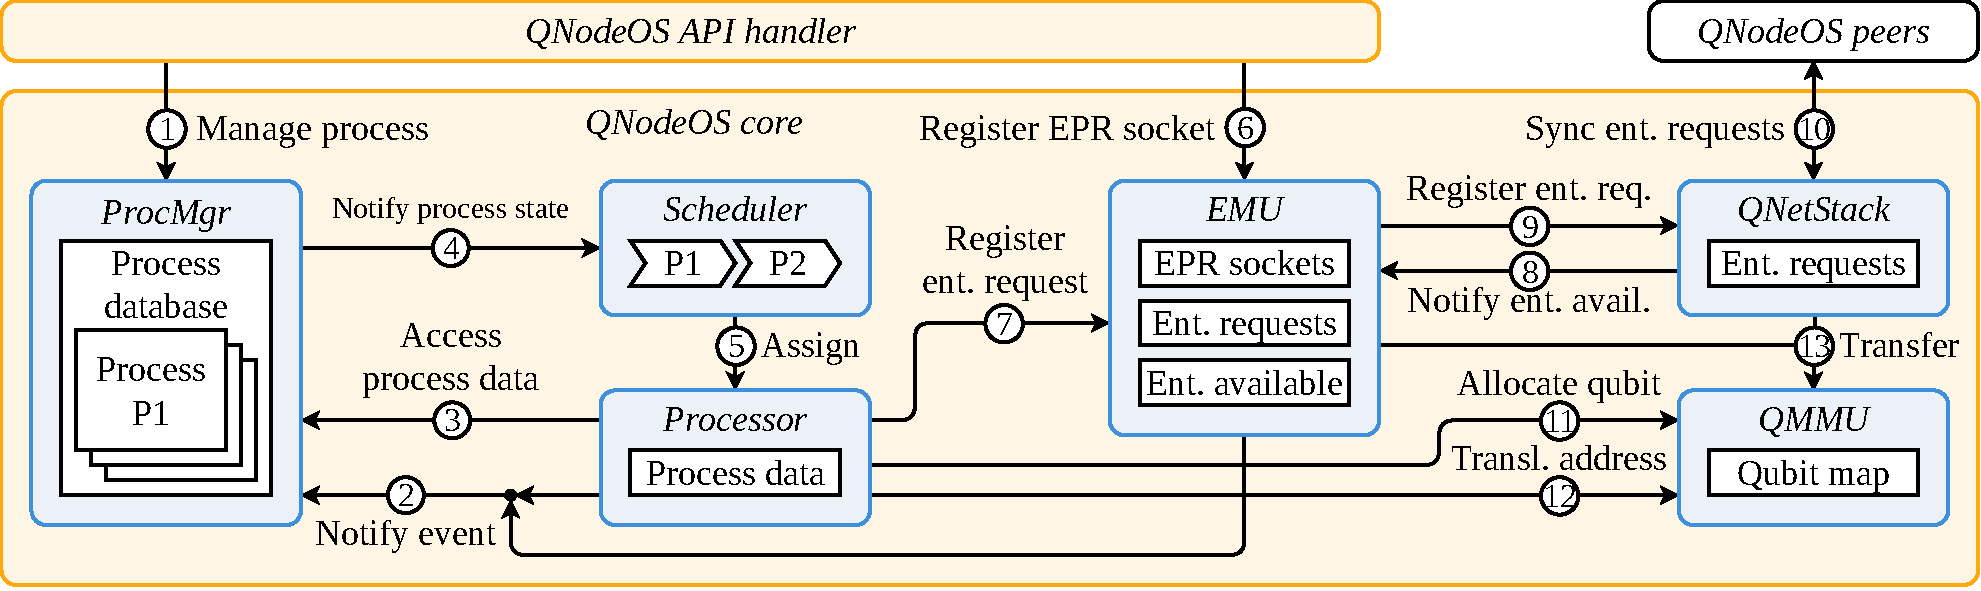
\includegraphics[width=\linewidth]{figures/qnodeos-core.pdf}
    \caption[]{
        \acrshort{qnodeos} core components and internal interfaces. The core layer includes:
        \begin{inlinelist}
            \item a \emph{process manager} (ProcMgr), which owns and manages access to
                  \acrshort{qnodeos} processes;
            \item a \emph{scheduler}, responsible for selecting the next process to be run;
            \item a \emph{processor}, which processes routines' instructions;
            \item an \emph{\acrlong{emu}} (\acrshort{emu}), which keeps a list of entanglement
                  requests and available entangled qubits;
            \item a \emph{quantum network stack} (QNetStack), whose responsibility is to coordinate
                  with peer nodes to schedule quantum networking instructions;
            \item a \emph{\acrlong{qmmu}} (\acrshort{qmmu}), which keeps a record of allocated
                  qubits.
        \end{inlinelist}
    }
    \label{fig:qnodeos-core}
\end{figure}

\section{Scheduler}

The \acrshort{qnodeos} scheduler registers processes that are ready to be scheduled, and assigns
them to the \acrshort{qnodeos} processor when the latter is available. Ready processes are stored in
a \emph{prioritized ready queue}, and processes of the same priority are scheduled with a
first-come-first-served policy.

\paragraph{Interfaces}

The scheduler only exposes one interface for process state notifications (interface~\circled{4} in
\cref{fig:qnodeos-core}), used by the process manager to signal when a process transitions to a new
state. When a \acrshort{qnodeos} process transitions to the ready state, it is directly added to the
scheduler's prioritized ready queue. When a process becomes idle, or is waiting for an event to
happen, the scheduler simply registers that the processor has become available.

\section{Processor}

The \acrshort{qnodeos} processor handles the execution of \acrshort{qnodeos} user and kernel
processes, by running classical instructions locally and issuing quantum instructions to the
\acrshort{qdevice} driver. While executing a process, the processor reads its routines and accesses
(reads and writes) its classical memory. The processor implements a specific instruction set
architecture dictated by the QASM language of choice.

\paragraph{Interfaces}

The processor exposes one interface for processor assignment (interface~\circled{5} in
\cref{fig:qnodeos-core}), used by the \acrshort{qnodeos} scheduler to activate the processor, when
it is idling, and assign it to a \acrshort{qnodeos} process.

\section{Entanglement Management Unit}

The \acrfull{emu} maintains a list of open \emph{EPR sockets} and a list of \emph{entanglement
requests}, and keeps track of the \emph{entangled qubits} produced by the quantum network stack.
Received entanglement requests are considered valid only if an EPR socket associated to such
requests exists. Valid requests are forwarded to the quantum network stack. Entangled qubit
generations are notified as events to the process manager.

\paragraph{Interfaces}

The \acrshort{emu} exposes interfaces for three services:
\begin{itemize}
    \item EPR socket registration (interface~\circled{6} in \cref{fig:qnodeos-core}): to register
          and open EPR sockets belonging to an application, and to set up internal classical network
          tables and to establish classical network connection.
    \item Entanglement request registration (interface~\circled{7} in \cref{fig:qnodeos-core}): to
          add entanglement requests to the list of existing ones, to be used when matching produced
          entangled qubits with a process that requested them.
    \item Entanglement notification (interface~\circled{8} in \cref{fig:qnodeos-core}): to register
          the availability of an entangled qubit, produced by the quantum network stack, and to link
          it to an existing entanglement request.
\end{itemize}

\section{Quantum Network Stack}

The quantum network stack on \acrshort{qnodeos} follows the model presented in
Ref.~\cite{dahlberg_2019_egp} which is based on the classical \acrshort{osi} network stack model for
separation of responsibilities. In particular, \emph{data link layer} and \emph{network layer}
protocols are part of the quantum network stack on \acrshort{qnodeos}. The \emph{physical layer} is
implemented on the \acrshort{qdevice}, the \emph{application layer} is part of the Host, and all
remaining layers are not currently part of the stack.

The quantum network stack component has an associated \emph{\acrshort{qnodeos} kernel process},
created statically on \acrshort{qnodeos}. However, this process's routine is dynamic: the
instructions to be executed on the processor depend on the outstanding entanglement generation
requests received from \acrshort{emu} and network peers.

\paragraph{Interfaces}

The quantum network stack exposes interfaces for two services:
\begin{itemize}
    \item Entanglement request registration (interface~\circled{9} in \cref{fig:qnodeos-core}): to
          add entanglement requests coming from the \acrshort{emu} to the list of existing ones,
          which are used to fill in the quantum network stack process's routine with the correct
          instructions to execute.
    \item Entanglement request synchronization (interface~\circled{10} in \cref{fig:qnodeos-core}):
          similar to the entanglement request registration interface, but to be used to synchronize
          (send and receive) requests with \acrshort{qnodeos} network peers.
\end{itemize}

\section{Quantum Memory Management Unit}

The \acrfull{qmmu} receives requests for \emph{qubit allocations} from \acrshort{qnodeos} processes,
and manages the subsequent usage of those. It also translates QASM \emph{virtual qubit addresses}
into physical addresses for the \acrshort{qdevice}, and keeps track of which process is using which
qubit at a given time. In general, a \acrshort{qmmu} should take into account that the topology of a
quantum memory determines what operations can be performed on which qubits, and thus allow processes
to allocate qubits of a specific type upon request. An advanced \acrshort{qmmu} could also feature
algorithms to move qubits in the background --- that is, without an explicit instruction from a
process's routine --- to accommodate an application's topology requirements while not trashing the
qubits being used by other \acrshort{qnodeos} processes. Such a feature could prove crucial to
increase the number of processes that can be using the quantum memory at the same time, and to
enhance multitasking performances.

\paragraph{Interfaces}

The \acrshort{qmmu} exposes interfaces for three services:
\begin{itemize}
    \item Qubit allocation and deallocation (interface~\circled{11} in \cref{fig:qnodeos-core}): a
          running process can ask for one or more qubits, which, if available, are allocated by the
          \acrshort{qmmu}, and their physical addresses are mapped to the virtual addresses provided
          by the requesting process.
    \item Virtual address translation (interface~\circled{12} in \cref{fig:qnodeos-core}): before
          sending quantum instructions to the \acrshort{qdevice} driver, the processor uses virtual
          qubit addresses specified in QASM to retrieve physical addresses from the \acrshort{qmmu},
          and then replaces virtual addresses with physical addresses in the instructions for the
          \acrshort{qdevice} driver.
    \item Qubit ownership transfer (interface~\circled{13} in \cref{fig:qnodeos-core}): qubits are
          only visible to the process that allocates them. However, in some cases, a process may
          wish to transfer some if its qubits to another one. A notable example is the quantum
          network process transferring an entangled qubit to the process that will use it.
\end{itemize}

\printbibliography[heading=subbibintoc,title={References}]
